\chapter{Thrust characteristics}

Graphs below present empirical data on the thrust produced by Sadulli Piccino and Sadulli Grosso. 
All data collected at normal conditions: standard atmospheric pressure (100 kPa) and normal temperature (25\degree{}C) at MSL.

\begin{ZubaxTableWrapper}{Propeller characteristics}
    \begin{ZubaxWrappedTable}{| X | X | X | X |}
    Parameter           & Sadulli Piccino   & Sadulli Grosso & Unit \\
    Propeller diameter  & 15                & 17             & inch \\
    Propeller pitch     & 5.5               & 6.2            & inch \\
\end{ZubaxWrappedTable}
\end{ZubaxTableWrapper}

In the realm of constant pitch propeller drives, there is a tendency for thrust efficiency reduction 
with the increase of propeller RPM. This means that although maximum thrust is limited by propeller material 
and motor and controller power limitations and may reach relatively high values,  
it may be beneficial not to use the drive at its maximum thrust levels and stay at relatively low RPM 
where the efficiency is higher. The specific efficiency level proposed for optimum operation is 10 gf/W. 
Aircraft designer should keep that in mind and select the propulsion system accordingly.

\newpage
\section{Sadulli Piccino thrust figures}

\begin{figure}[!hbt]
    \centerline{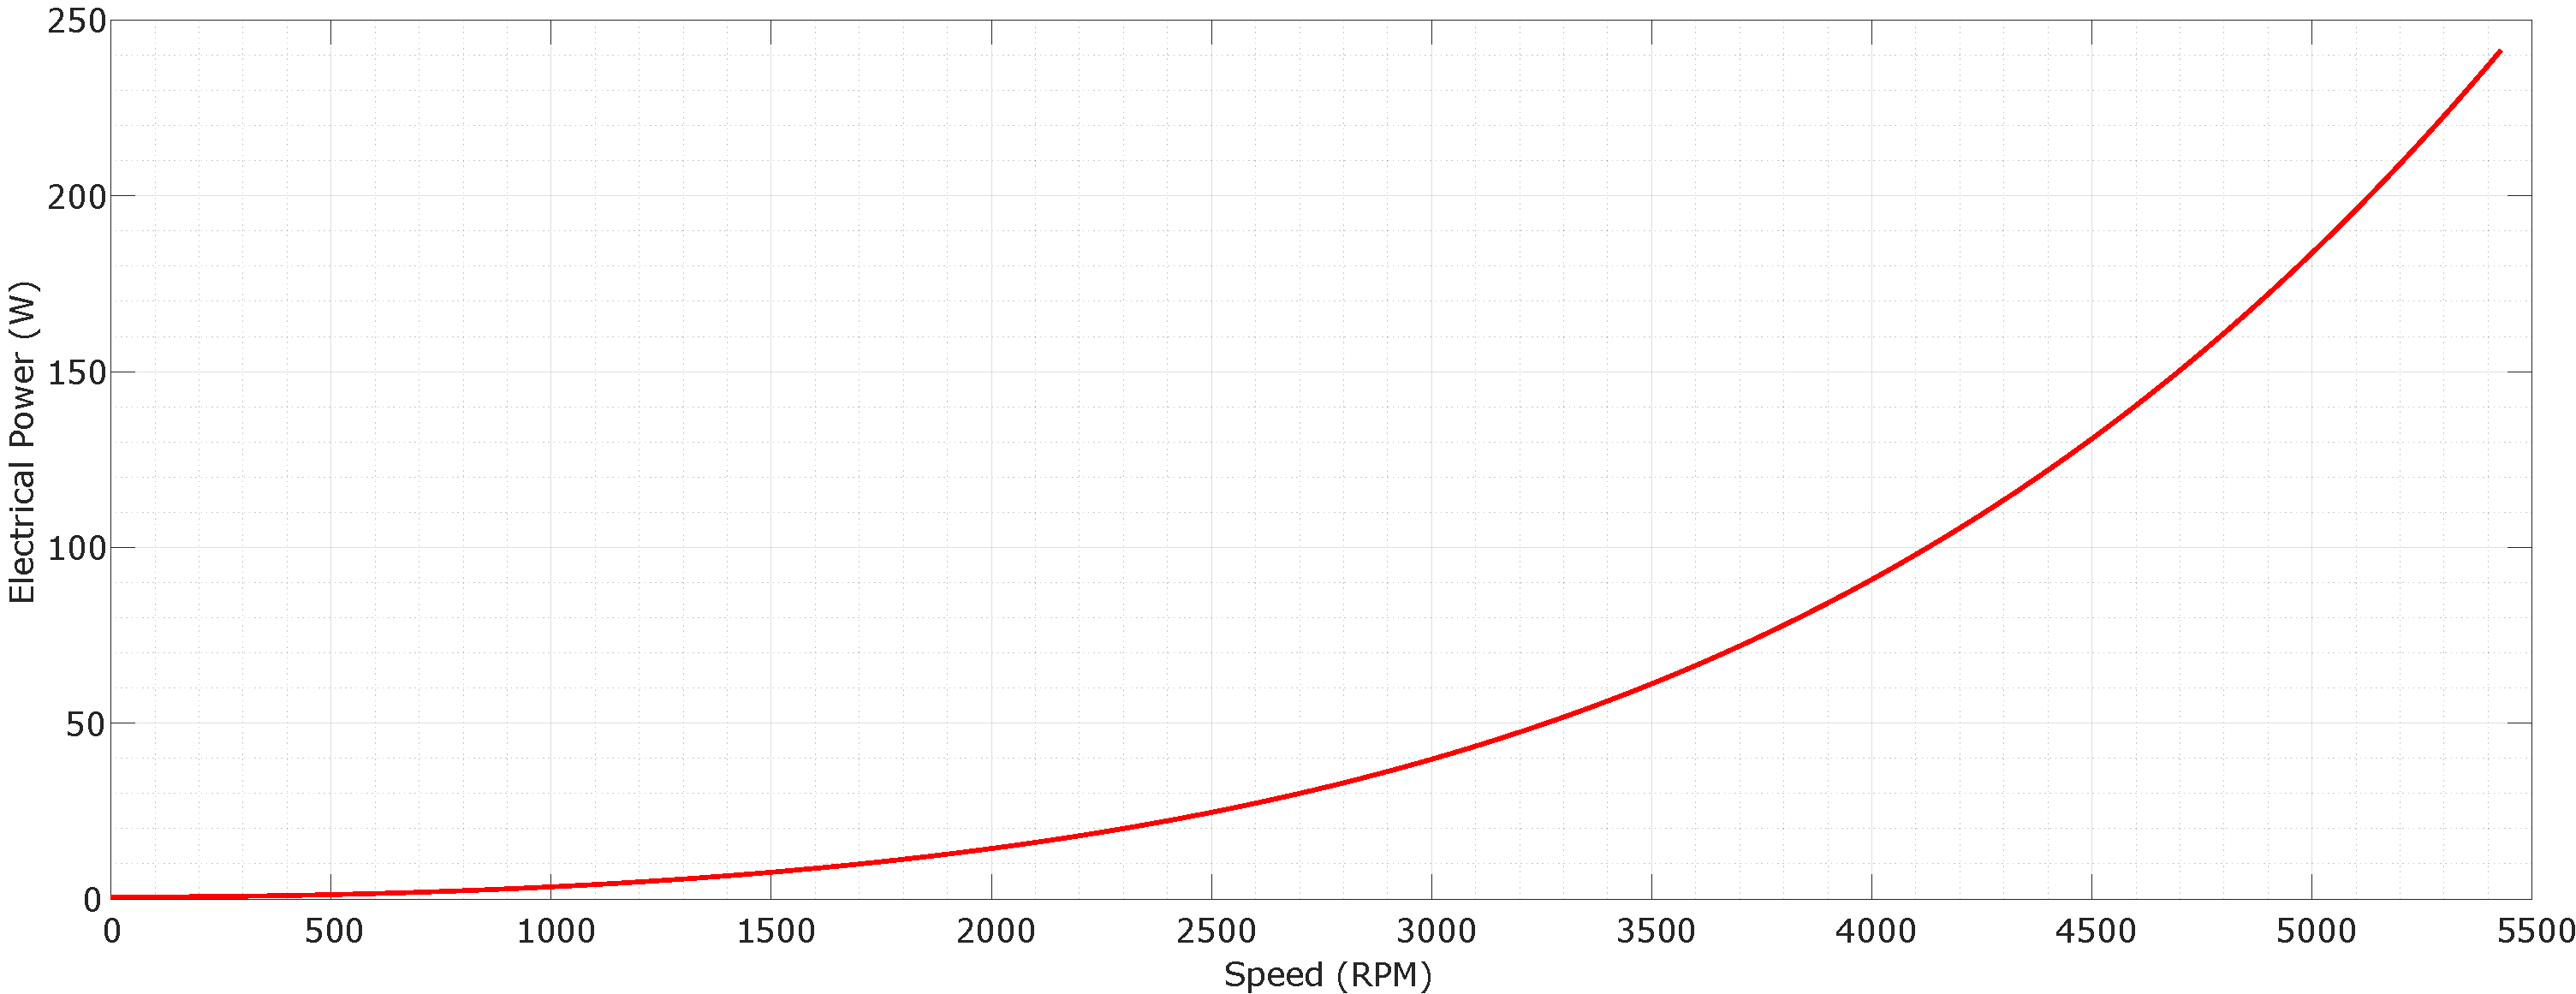
\includegraphics[width=1\textwidth]{figures/thrust_graphs/piccino_power-rpm.pdf}}
    \caption{Sadulli Piccino electrical power vs. RPM}
\end{figure}

\begin{figure}[!hbt]
    \centerline{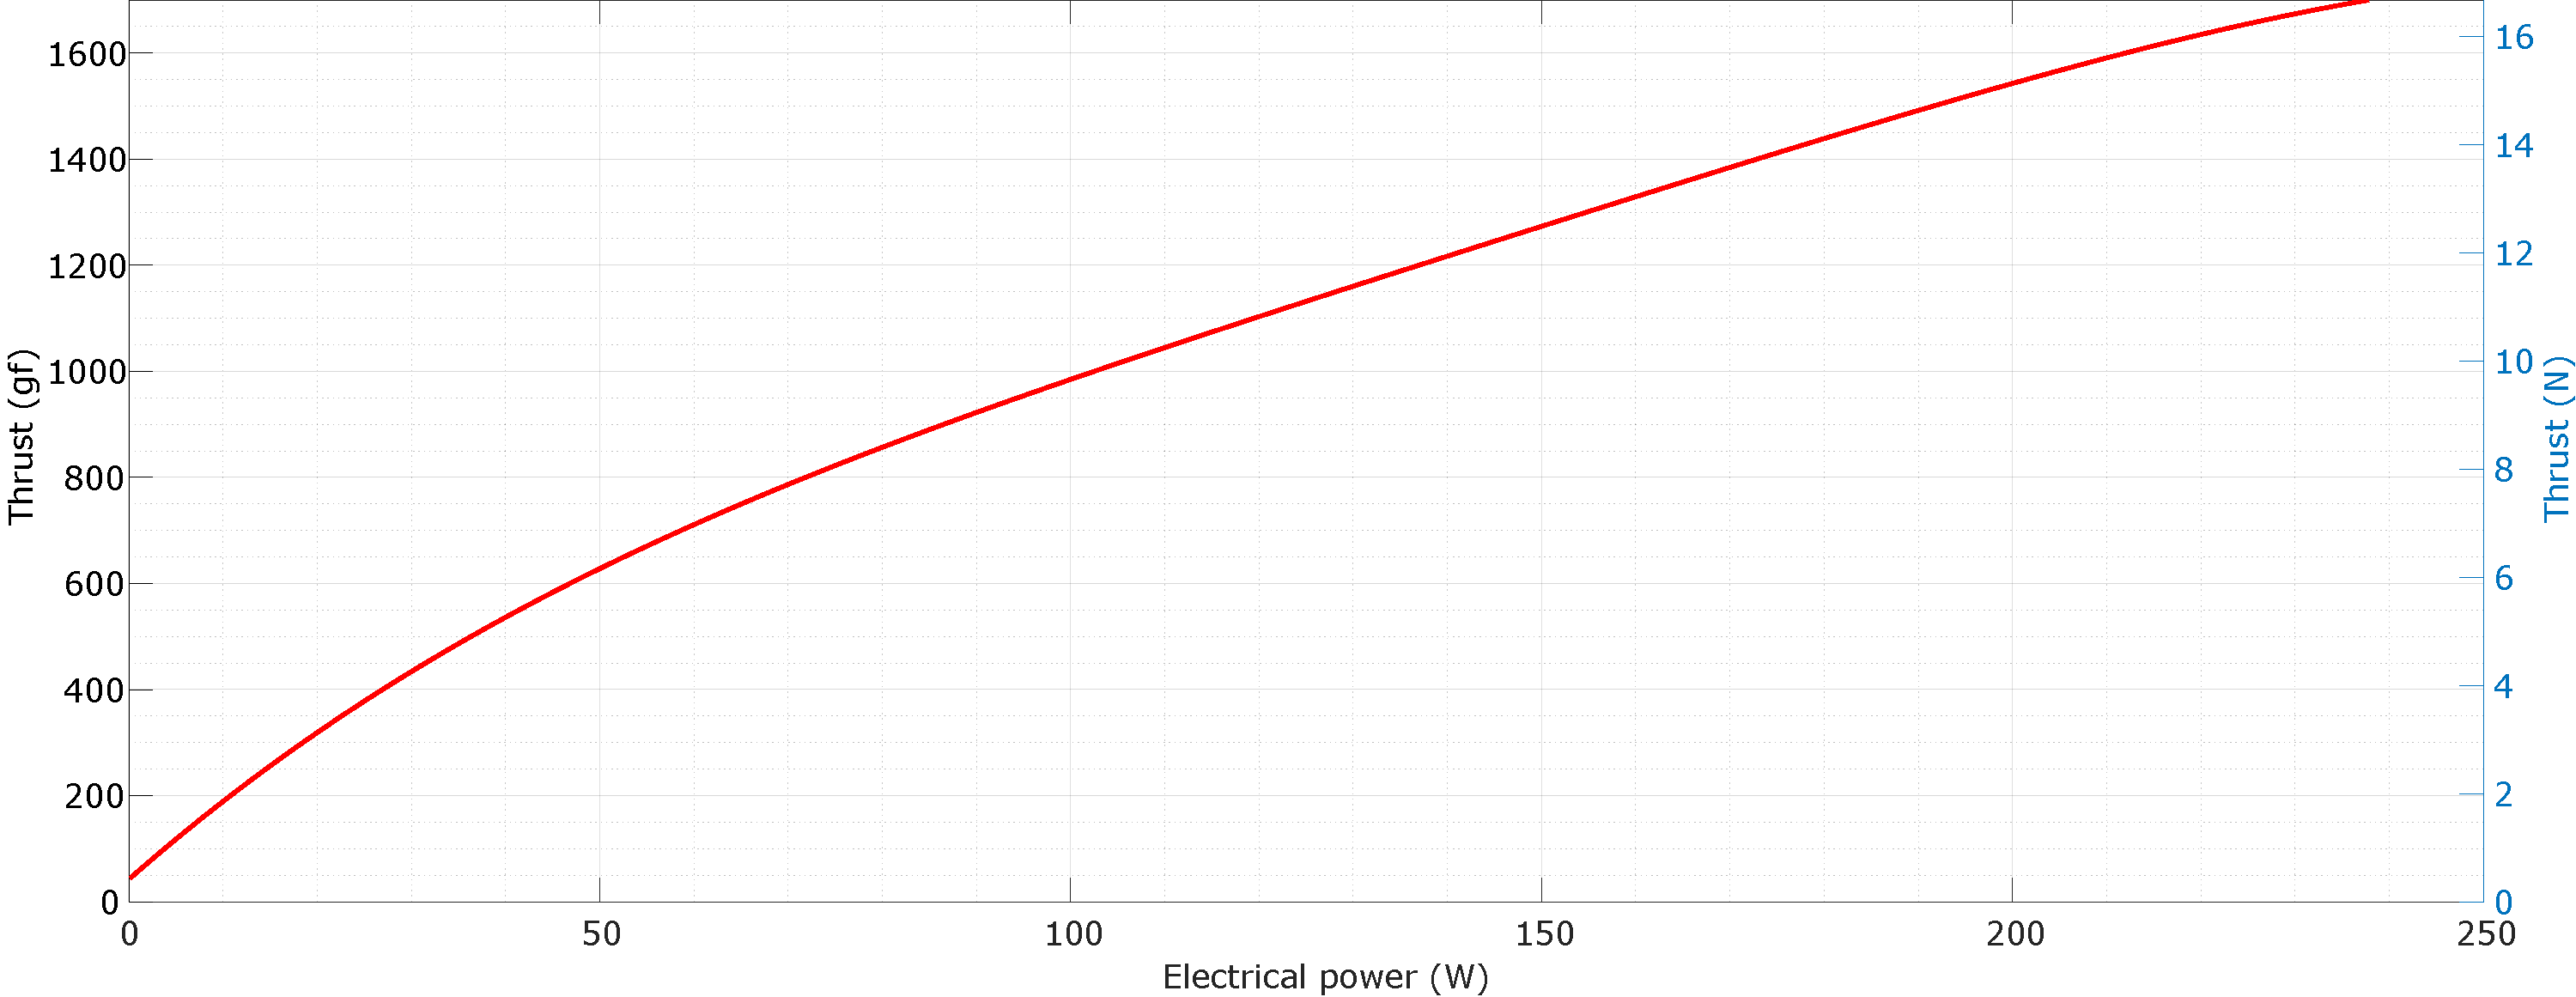
\includegraphics[width=1\textwidth]{figures/thrust_graphs/piccino_thrust-power.pdf}}
    \caption{Sadulli Piccino thrust  vs. electrical power}
\end{figure}

\begin{figure}[!hbt]
    \centerline{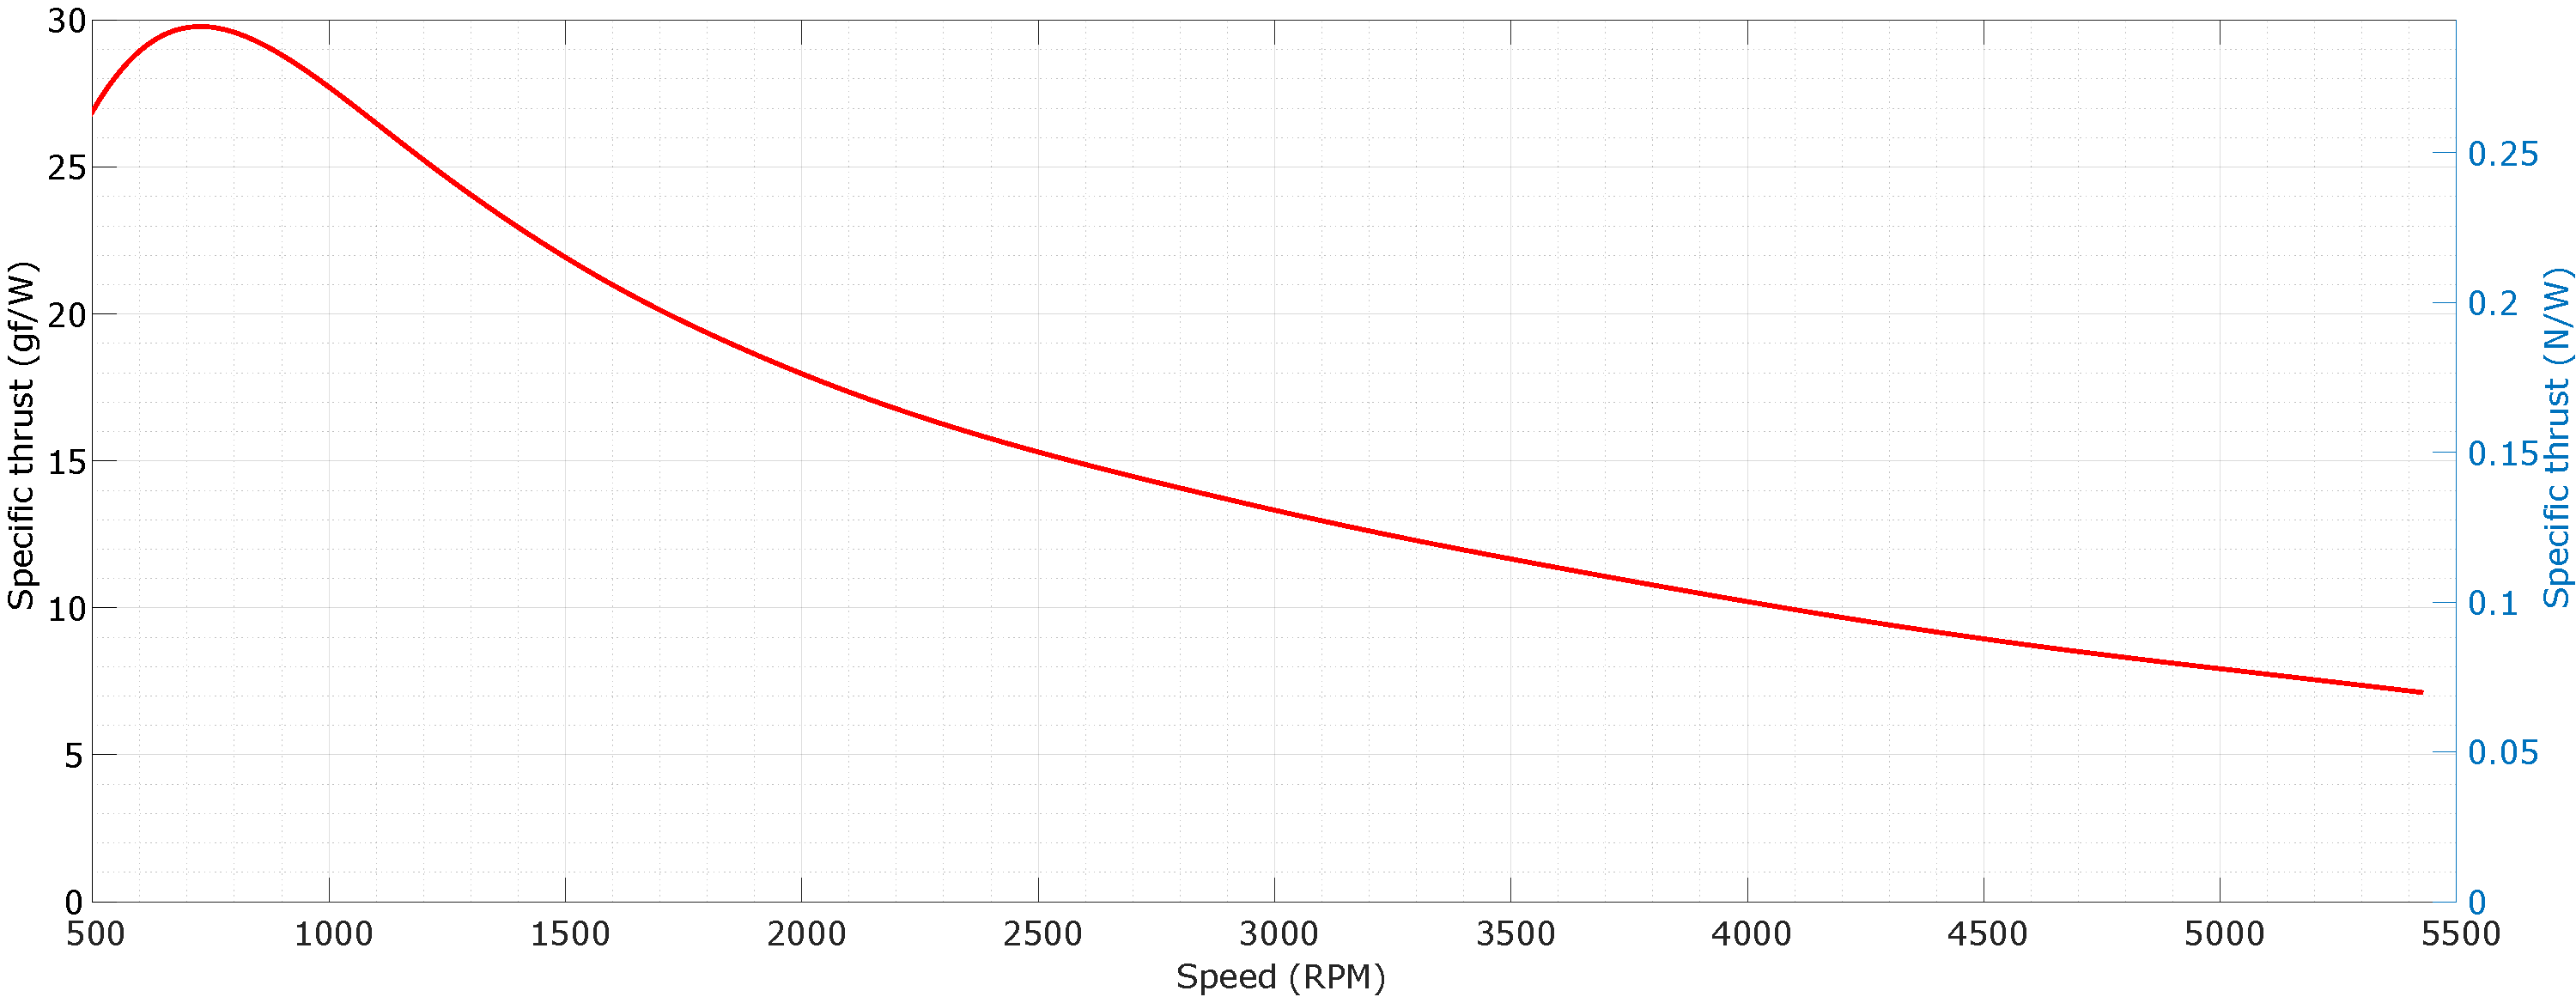
\includegraphics[width=1\textwidth]{figures/thrust_graphs/piccino_specific_thrust-rpm.pdf}}
    \caption{Sadulli Piccino specific thrust vs. RPM}
\end{figure}

\newpage

\section{Sadulli Grosso thrust figures}

\begin{figure}[!hbt]
    \centerline{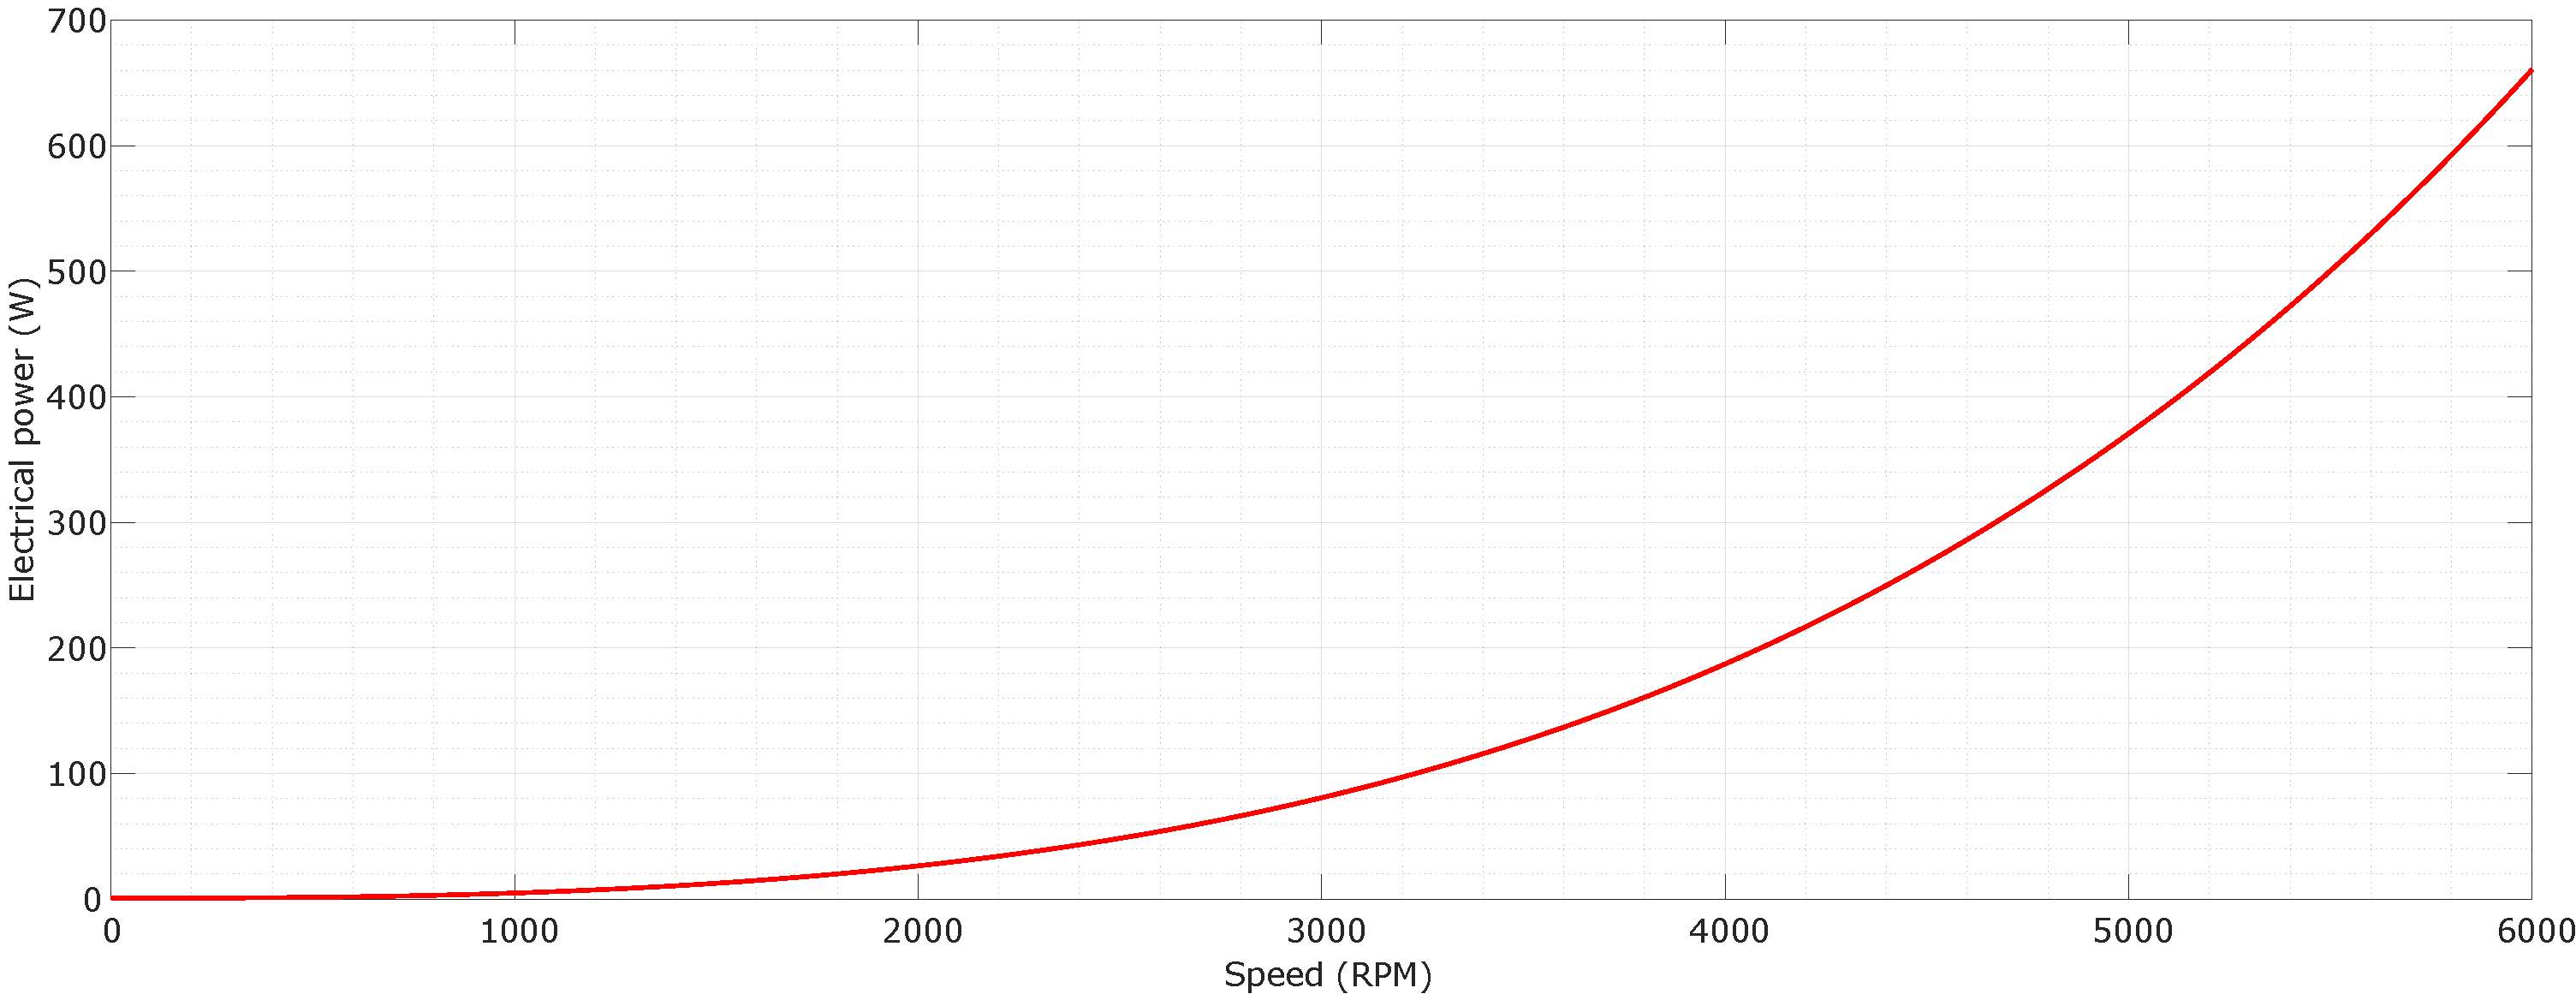
\includegraphics[width=1\textwidth]{figures/thrust_graphs/grosso_power-rpm.pdf}}
    \caption{Sadulli Grosso electrical power vs. RPM}
\end{figure}

\begin{figure}[!hbt]
    \centerline{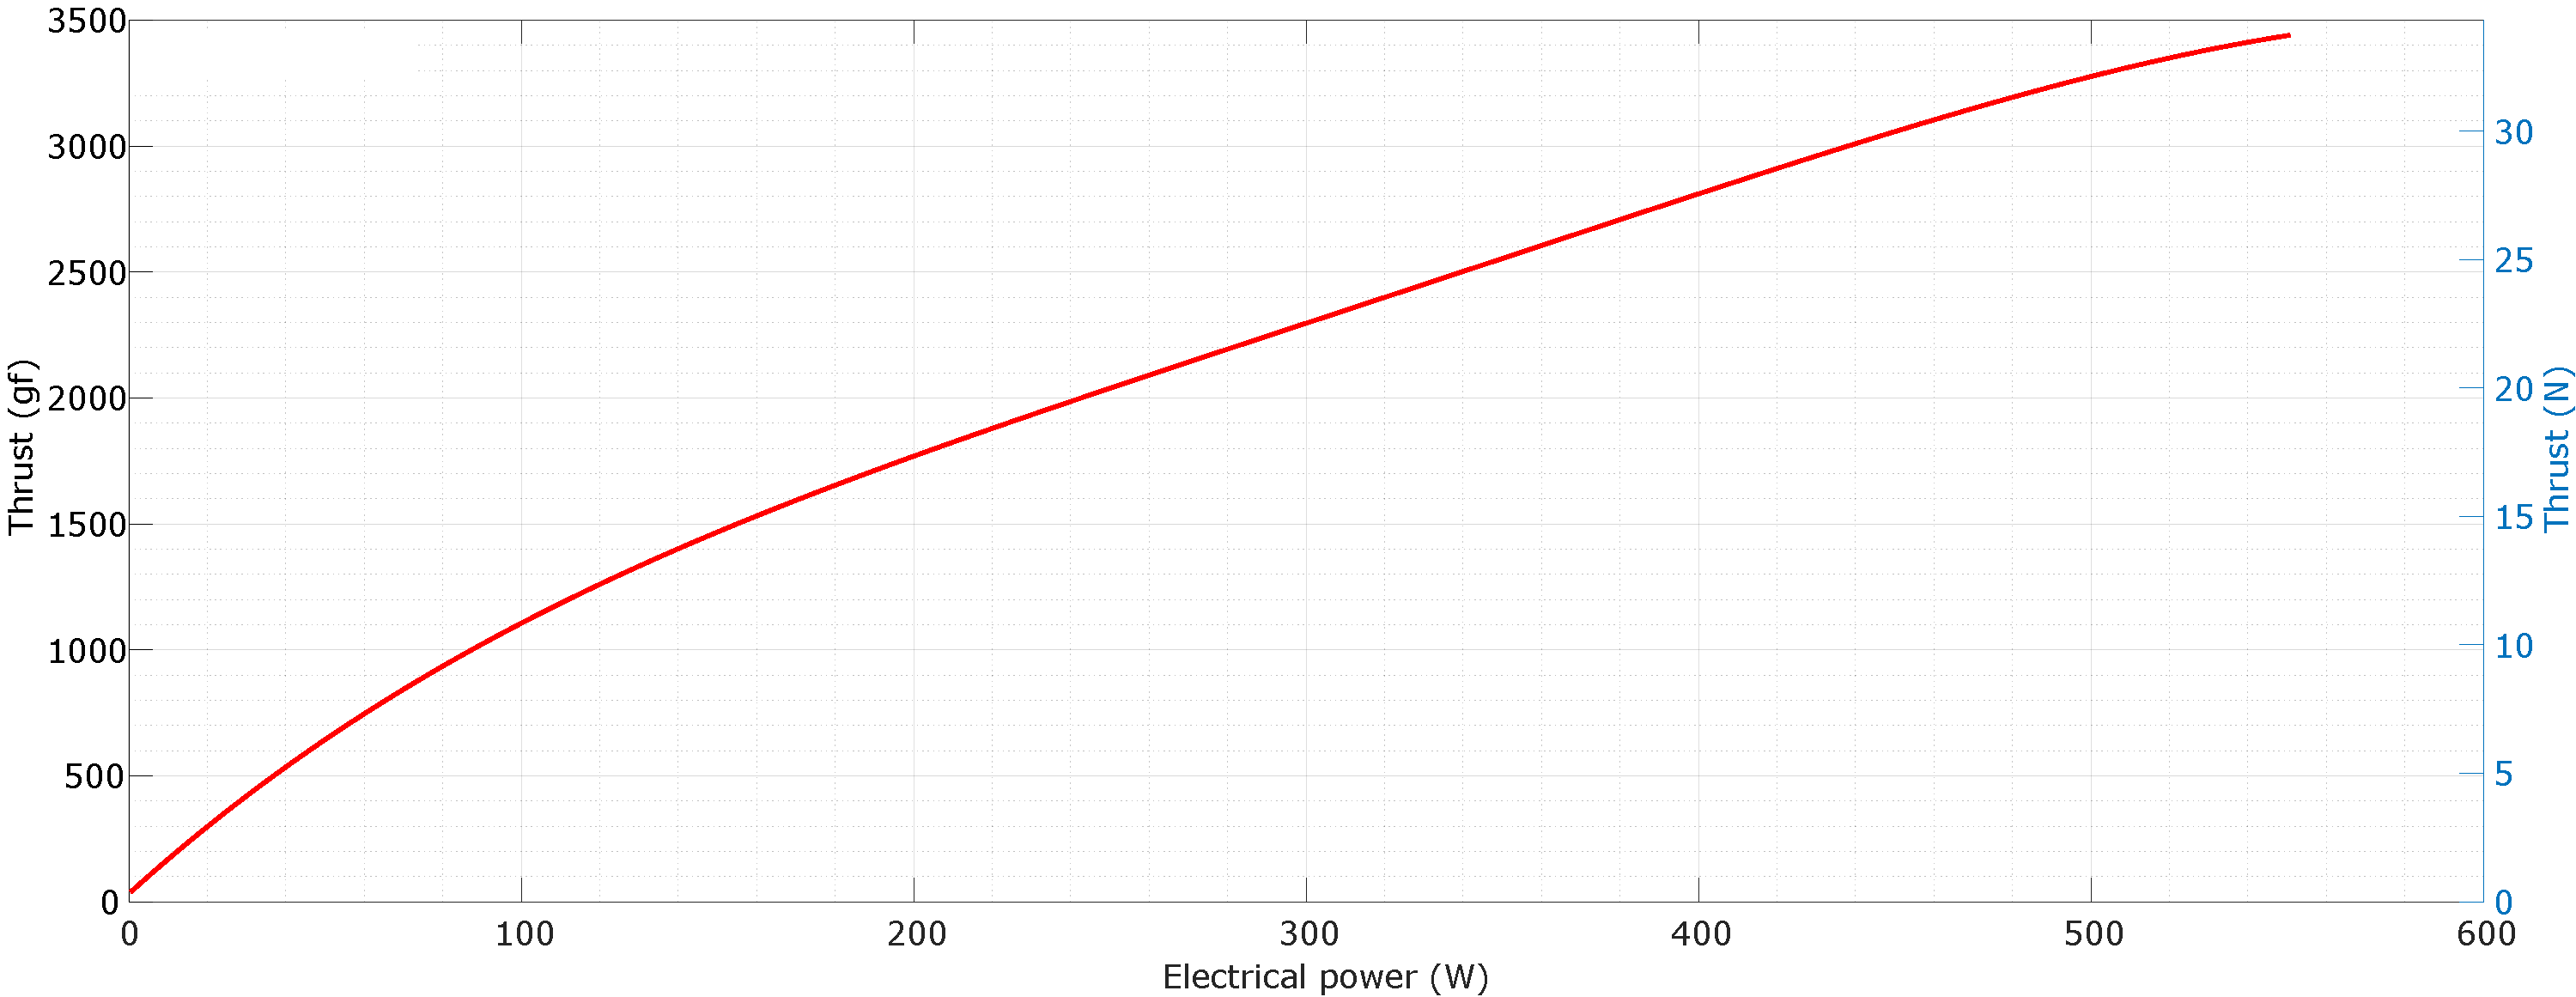
\includegraphics[width=1\textwidth]{figures/thrust_graphs/grosso_thrust-power.pdf}}
    \caption{Sadulli Grosso thrust  vs. electrical power}
\end{figure}

\begin{figure}[!hbt]
    \centerline{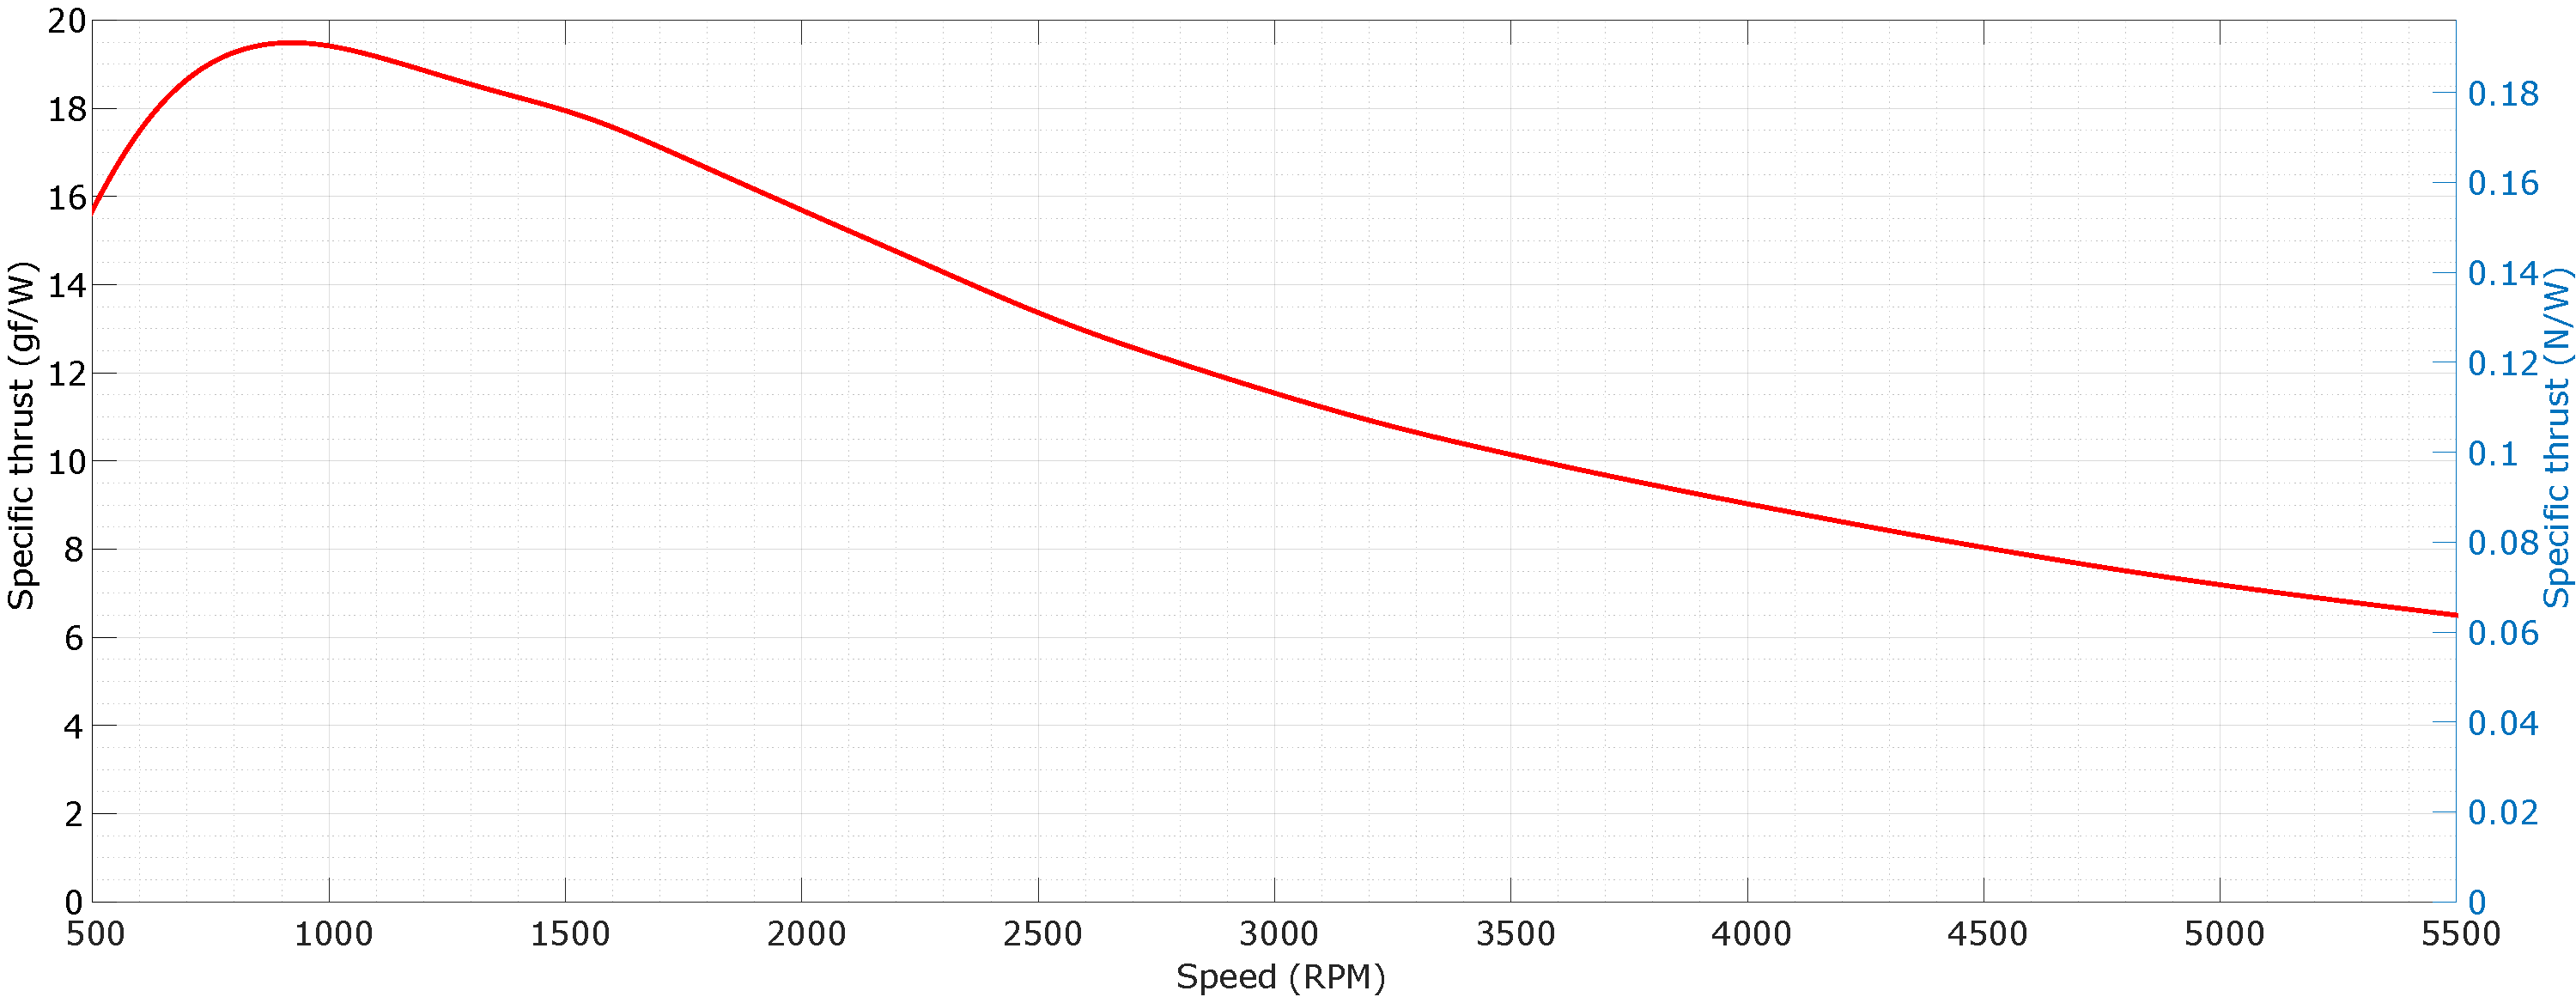
\includegraphics[width=1\textwidth]{figures/thrust_graphs/grosso_specific_thrust-rpm.pdf}}
    \caption{Sadulli Grosso specific thrust vs. RPM}
\end{figure}